\documentclass[a4paper, 12pt]{article}

\usepackage[T2A]{fontenc}
\usepackage[utf8]{inputenc}
\usepackage[english,russian]{babel}
\usepackage{amsmath, amsfonts, amssymb, amsthm, mathtools}

\usepackage{indentfirst}
\usepackage{icomma}
\usepackage{hyperref}
\usepackage{soulutf8}

\usepackage{multirow}
\usepackage{hhline}
\usepackage{graphicx}

\usepackage{tikz}
\usetikzlibrary{calc}

\usepackage{diagbox}
\usepackage{wrapfig}
\usepackage{caption}
\usepackage{subcaption}

\usepackage{geometry}
\geometry{top=25mm}
\geometry{bottom=30mm}
\geometry{left=20mm}
\geometry{right=20mm}

\renewcommand{\epsilon}{\varepsilon}
\renewcommand{\phi}{\varphi}
\newcommand{\mean}[1]{\left<#1\right>}

\title{\textbf{Работа 1.4.1}\linebreak Изучение физического маятника}
\author{Константин Ерёмин Б03-204}
\date{Декабрь 2022}

\begin{document}
    \maketitle

    \section{Введение}
        \begin{target}
            исследовать вынужденную прецессию гироскопа; установить зависимость скорости вынужденной прецесии от величины момента сил, действующих на ось гироскопа; определить скорость вращения ротора гироскопа и сравнить её со скоростью, рассчитанной по скорости прецесии.
        \end{target}

        \begin{setting}
            гироскоп в карданном подвесе, секундомер, набор грузов, отдельный ротор гироскопа. цилиндр известной массы, крутильный маятник, штангенциркуль, линейка.
        \end{setting}

    \section{Теоретическое описание работы}
        Вращение гироскопа, обладающего моментом импульса $\vec L$ и угловой скоростью вращения его оси $\vec \Omega$ (\emph{скорость прецесии}), описывается уравнением
        \[\frac{d\vec{L}}{dt} = \vec \Omega \times \vec L, \text{ где } \frac{d\vec{L}}{dt} = \vec M.\]
        $\vec M$ "--- момент сил, приложенный к оси маховика.

        Для гироскопа с закреплённым на оси на расстоянии $l$ от центра подвеса грузом массой $m$ скорость прецесии равна
        \[\Omega = \frac{mgl}{I_z\omega_0},\]
        где $I_z$ "--- один из главных моментов инерции, $\omega_0$ "--- угловая скорость вращения маховика, причём для гироскопа $I_z \omega_0 \gg I_x \omega_x, I_y \omega_y$.
        
        Для определения момента инерции ротора гироскопа используется отдельный ротор неиспользуемого гироскопа. Измеряются крутильные колебания ротора-копии, период которых зависит от момента инерции $I_0$ и модуля кручения проволоки $f$:
        \begin{equation}
            T_0 = 2\pi \sqrt{\frac{I_0}{f}}.    
        \end{equation}
        Чтобы исключить модуль кручения проволоки, вместо ротора гироскопа к той же проволоке подвешивают цилиндр изместных массы и диаметра. Его момент инерции равен $I_\text{ц} = \frac{md^2}{8}$ После исключения $f$ получаем:
        \begin{equation}
            I_0 = I_\text{ц} \frac{T_0^2}{T_\text{ц}^2}.
            \label{eq:inertia}
        \end{equation}

		\begin{figure}
			\centering
			\begin{minipage}{0.4\textwidth}
				\centering
				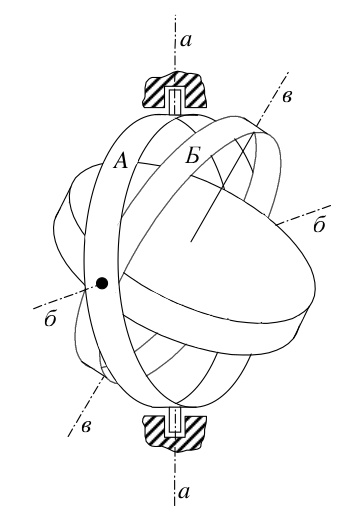
\includegraphics[width=0.9\linewidth]{gyro.png}
				\caption{Гироскоп в карданном подвесе}
				\label{fig:gyro}
			\end{minipage}\hfill
            \begin{minipage}{0.6\textwidth}
				\centering
				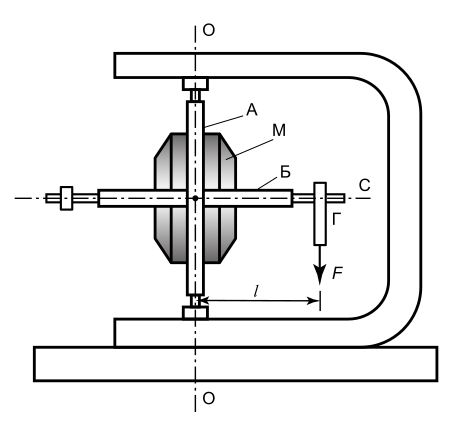
\includegraphics[width=0.9\linewidth]{setting.png}
				\caption{Схема экспериментальной установки}
				\label{fig:setting}
			\end{minipage}
        \end{figure}

        Также скорость вращения ротора можно определить с помощью осциллографа. Статор гироскопа имеет две обмотки, одна из которых раскручивает гироскоп, в другой обмотке, неподвижной(?), ротор наводит переменную ЭДС, частоты которой близка к частоте вращения. Частоту ЭДС можно измерить по фигурам Лиссажу: при совпадении частот получаем на экране эллипс.

    \section{Ход работы}
        После включения питания ротор раскручивается до максимальной скорости в течение 4-5 минут. При лёгком постукивании по оси гироскоп покоится, а при подвешивании груза Г к рычагу С (см. рис. \ref{fig:setting}) наблюдается прецессия. Трение в оси приводит к тому, что рычаг опускается.

        На ось гироскопа будем закреплять различные грузы и тем самым, измеряя периоды прецесии, получим зависимость $\Omega\left(M\right)$ (таблица \ref{table:periods} и рисунок \ref{fig:omega}). По методу наименьших квадратов находим $\left(I_z w_0\right)^{-1}$.

        Для оценки погрешности $\left(I_z w_0\right)^{-1}$ по $\Omega$ и $M$ примем погрешность измерения периода прецессии равной 0.5 секунды. Тогда полная погрешность складывается из случайной (по МНК), погрешности измерения периода и массы груза:  
        \begin{equation*}
            \sigma_k \approx k \sqrt{\frac{0.0001}{0.0589}^2 + \frac{0.5}{60}^2 + \frac{1}{100}^2} = k \cdot 0.013 = 0.773 \times 10^{-3}
        \end{equation*}

        \begin{table}
            \centering
            \begin{tabular}{|l||c|c|c|c|c|c|}
                \hline
                $m = 93$ гр & $T$, c & 106.14 & 110.27 & 110.24 & 110.17 & 110.13 \\
                \hline
                $m = 142$ гр & $T$, c & 71.77 & 71.22 & 71.52 & 71.39 & 71.46 \\
                \hline
                $m = 173$ гр & $T$, c & 59.02 & 59.12 & 59.55 & 59.54 & 59.22 \\
                \hline
                $m = 215$ гр & $T$, c & 47.18 & 47.24 & 47.40 & 47.28 & 47.34 \\
                \hline
                $m = 268$ гр & $T$, c &37.69 & 37.62 & 37.48 & 37.64 & 37.67 \\
                \hline
                $m = 338$ гр & $T$, c & 30.09 & 30.15 & 30.02 & 30.08 & 30.07 \\
                \hline
            \end{tabular}
            \caption{Измерение периодов прецессии при различных приложенных моментах}
            \label{table:periods}   
        \end{table}

        \begin{figure}
            \centering
            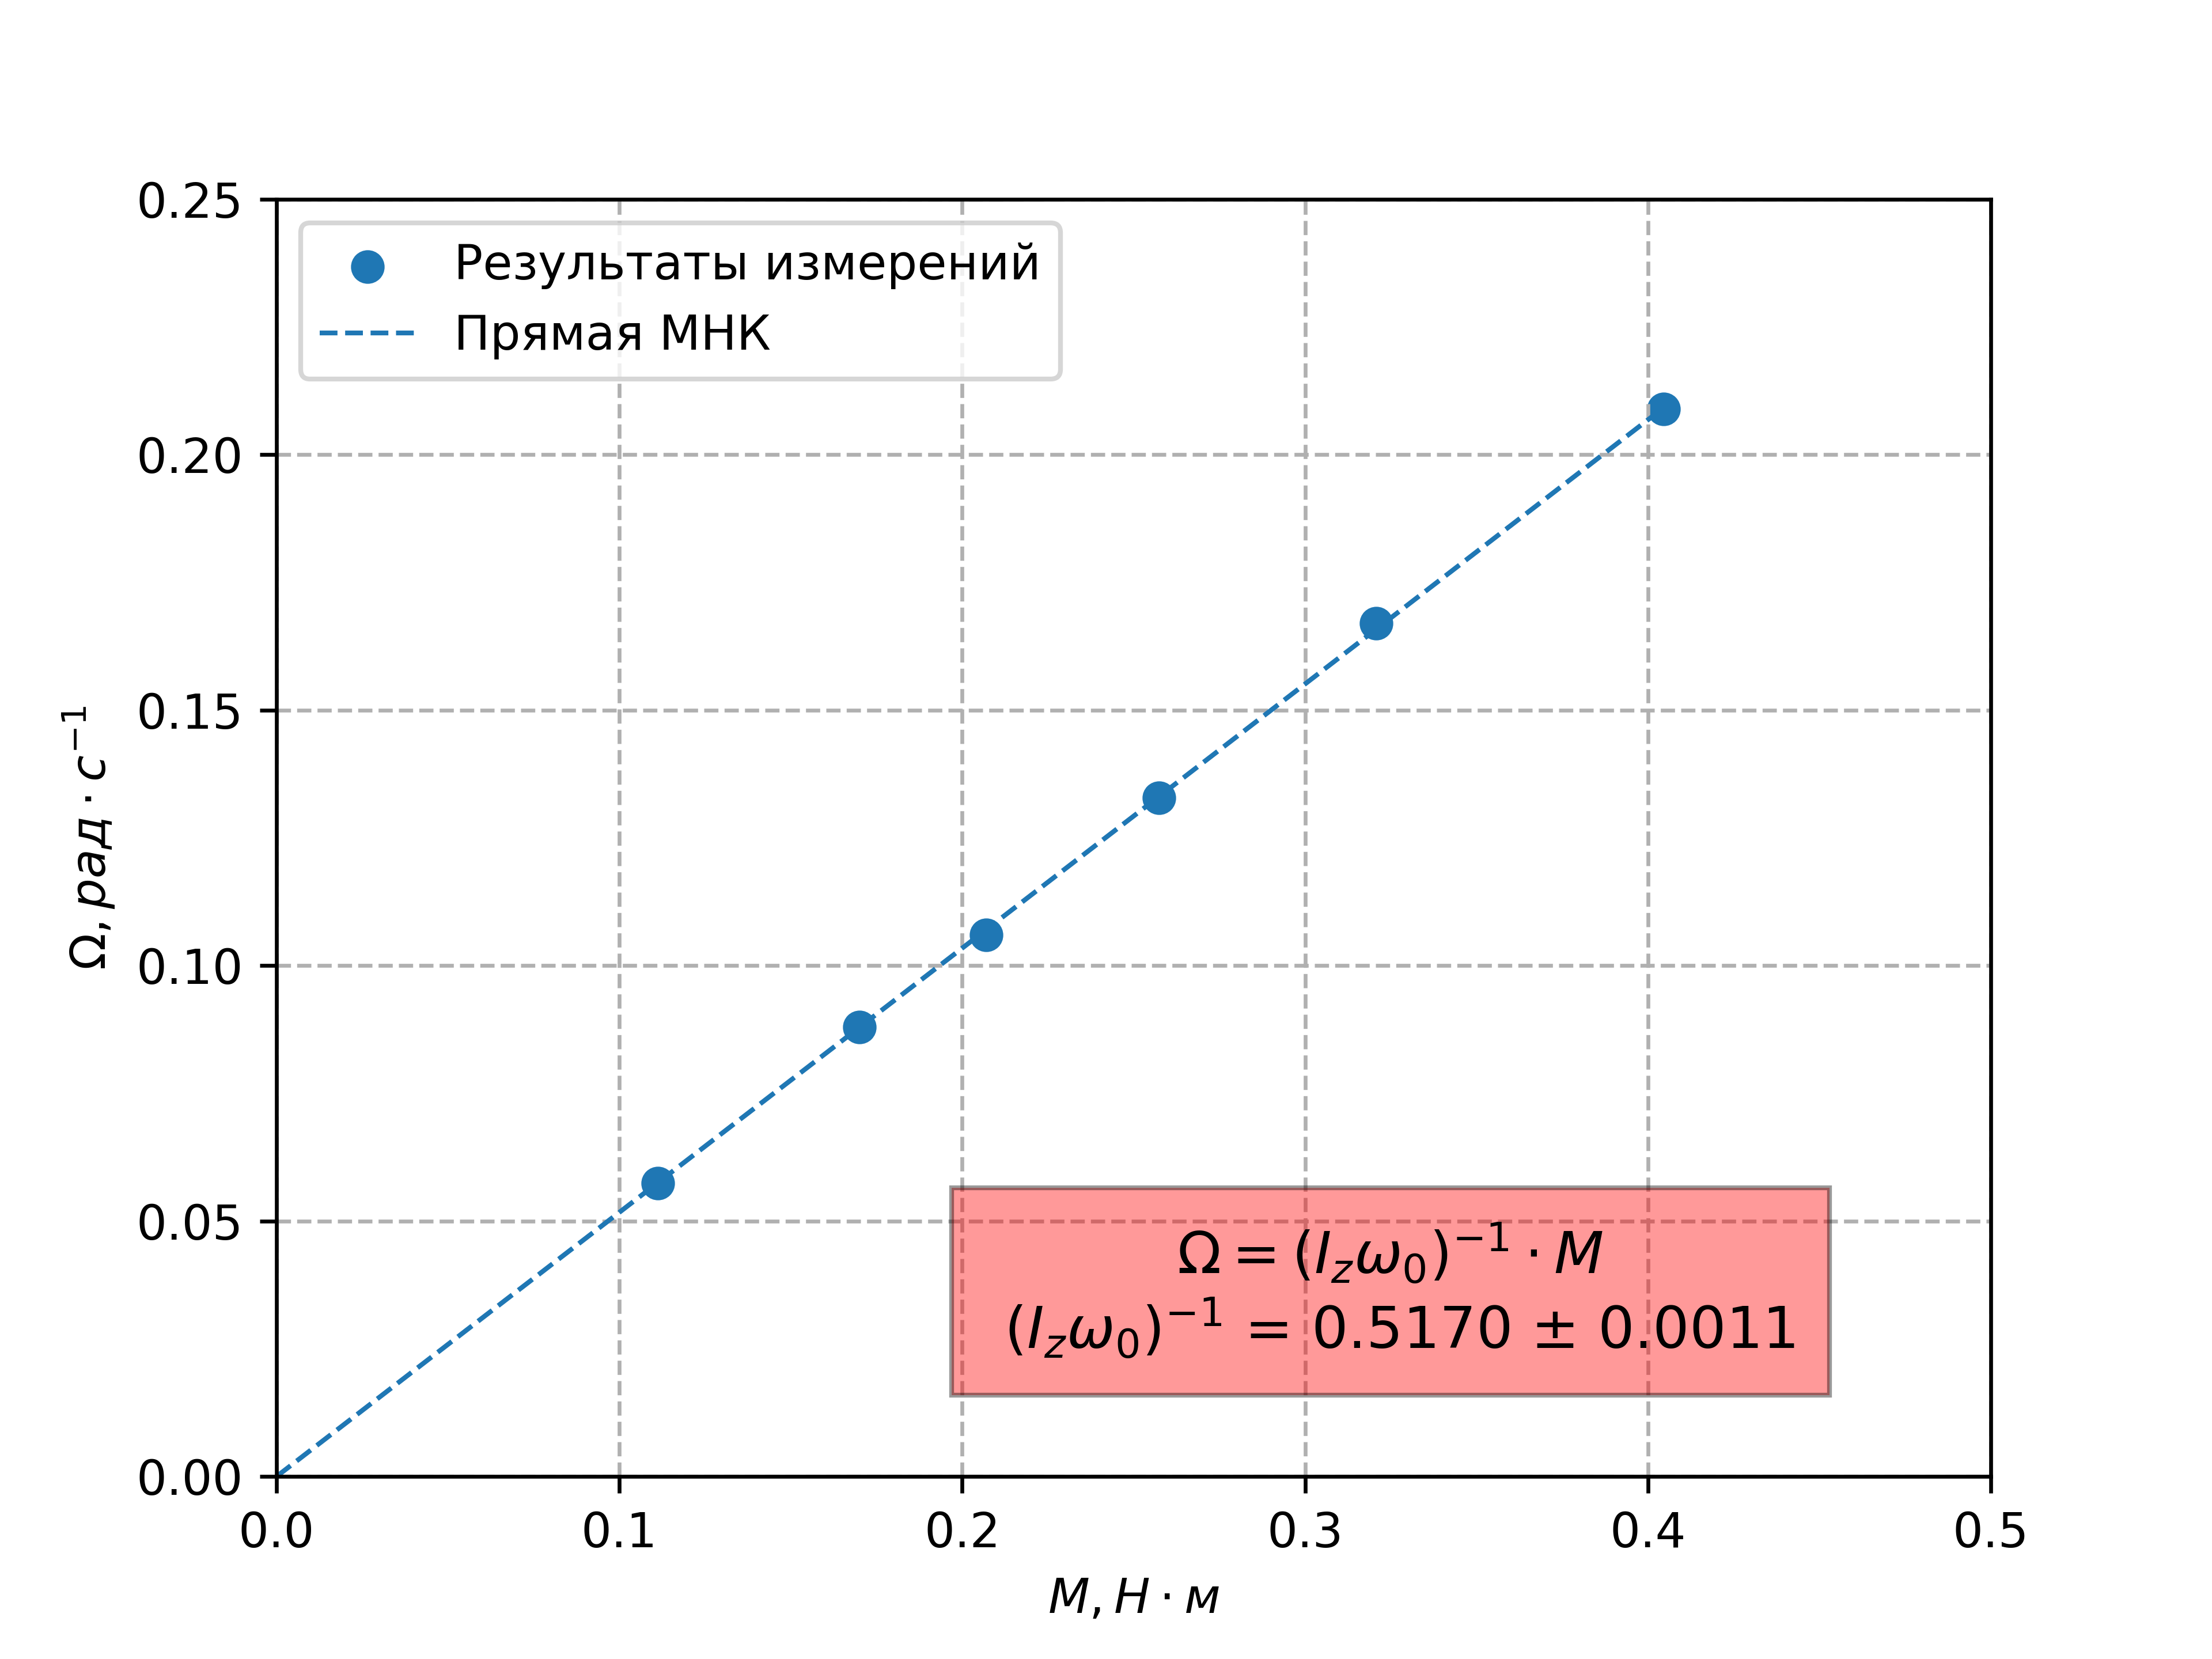
\includegraphics[width=0.75\linewidth]{Omega-M.png}
               \caption{График $\Omega\left(M\right)$}
               \label{fig:omega}
        \end{figure}

        \begin{table}
            \centering
            \begin{tabular}{|l|c|c|c|c|c||r|}
                \hline
                $T_\text{цилиндр}$, c & 4.050 & 4.054 & 4.053 & 4.047 & - & $T = 4.051 \pm 0.003$ c\\
                \hline
                $T_\text{ротор}$, c & 3.244 & 3.103 & 3.225 & 3.210 & 3.230 &  $T = 3.202 \pm 0.057$ c\\
                \hline
            \end{tabular}
            \caption{К измерению $I_0$ ротора}
            \label{table:rotor}
        \end{table}

        \pagebreak

        Найдём момент инерции ротора $I_0$ по формуле \ref{eq:inertia}. Для этого найдём периоды колебаний ротора и цилиндра (таблица \ref{table:rotor}), момент инерции цилиндра $I_\text{ц} = \frac{md^2}{8} = 1.223\times10^{-3} \cdot \text{кг м}^2$. Получаем, что $I_0 = \left(0.768 \pm 0.014\right) \times10^{-3} \cdot \text{кг м}^2$.

        Находим, наконец, частоту вращения ротора:
        \[\nu = \frac{\omega_0}{2\pi} = \frac{1}{2\pi \cdot 0.517 \cdot 0.000768} = 400.84 \text{ Гц}\]
        Погрешность:
        \[\sigma_\nu = \nu * \sqrt{\frac{0.014}{0.768}^2 + 0.013^2} = 6.8\text{ Гц}\]

        Теперь определим частоту ротора с помощью осциллографа: подключим его к гироскопу и подберём такую частоту генератора, подключённого ко второму входу осциллографа, чтобы на экране появилась фигура Лиссажу, а именно эллипс.
        С включённым двигателем гироскопа частота получается равной 400 Гц, что совпадает в пределах погрешностей с полученным ранее.
        Однако включённый двигатель наводит токи в обмотке, с помощью которой мы измеряем частоту вращения маховика, и на самом деле на осциллографе мы можем получить частоту тока, а не вращения.
        Если отключить двигатель и тут же, пока Вращение не замедлилось, измерить частоту, то она будет равной 389 Гц, что уже не попадает в погрешность измеренной нами чатоты.

    \section{Вывод}
        В ходе работы двумя способами была определа частота вращения маховика гироскопа в карданном подвесе.
        \begin{itemize}
            \item С помощью измерений периода прецесии: $\nu = 400.8 \pm 6.8$ Гц
            \item С помощью осциллографа: $\nu = 389$ Гц
        \end{itemize}

\end{document}